\chapter[Materiais e Métodos]{Materiais e Métodos}

Utilizou-se das metodologias de pesquisa e escolha dos componentes que serão utilizados para desenvolvimento do sistema. Neste trabalho, nos atentaremos a propor o sistema embarcado capaz de realizar as operações necessárias para cumprir os objetivos descritos na Seção \ref{OBJETIVOS}.

Na busca de uma solução para o sistema proposto, desmembrou-se o diagrama (Figura \ref{fig:blocos}) a fim de modularizar o processo. Primeiramente, a aquisição do vídeo e a codificação dos dados para envio (definições das especificações de comunicão, tais como número de portadoras, tipo de modulação, codificação de linha e canal) não seram tratados neste trabalho, assim como a recepção e decodificação desses dados. 


\begin{figure}[h]
	\centering
	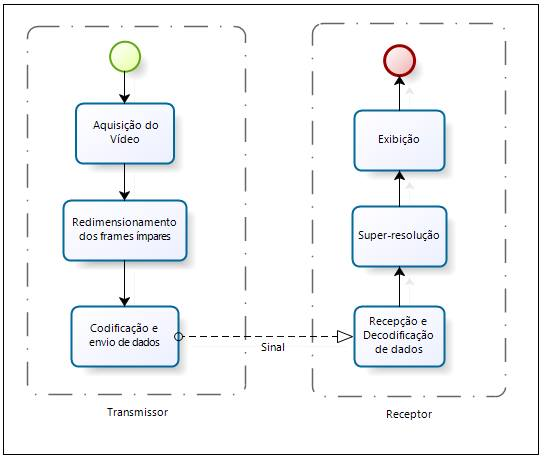
\includegraphics[scale=.7]{figuras/diagrama_blocos_solucao.jpg}
	\caption{Diagrama de blocos proposto para solução.}
	\label{fig:blocos}
\end{figure}
\section{Transmissor}

Para o transmissor, escolheu-se o \textit{kit} de desenvolvimento \textit{Raspberry Pi 2 Model B}. O \textit{Raspberry Pi 2} é um dos dispositivos mais populares atualmente entre estudantes, profissionais e hobbistas da área de Eletrônica. Segundo, o próprio site da \textit{Raspberry Pi
Foundation} \cite{raspberryOrg}, o dispositivo é um computador do tamanho de um cartão de crédito, de baixo custo, capaz de se concectar a um monitor de computador ou televisão e é capaz ,através de um cartão de memória SD, rodar um sistema operacional baseado em Linux, sendo
um dos mais populares o Raspbian (distribuição Debian voltada especificamente para o
Raspberry Pi).

A capacidade de rodar sistemas operacionais baseados em distribuições Linux, nos dá a possibilidade de utilizar \textit{frameworks} não
é a única razão pela qual o Raspberry Pi é amplamente utilizado